\documentclass{standalone}
\usepackage{tikz}
\usetikzlibrary{angles,quotes, calc}
\usepackage{amsmath}
\usepackage{amssymb}

% Define custom commands for better formatting
\newcommand{\matr}[1]{\mathbf{#1}}
\newcommand{\expect}[1]{\mathbb{E}\left[#1\right]}

\begin{document}
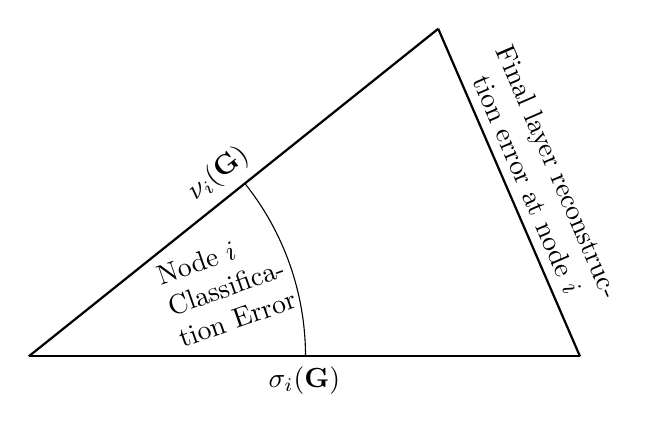
\begin{tikzpicture}[scale=2]
    \def\slope{0.8}
    \def\xA{3.5}
    \def\yA{0}
    \def\xB{2.6}
    \def\yB{\xB * \slope}
    \pgfmathsetmacro{\etaValue}{atan(\slope)}
    
    %\pgfmathsetmacro{\slope}{\rhovalue/sqrt(1-\rhovalue^2)}
    % Define the vertices of the triangle
    \coordinate (O) at (0,0);
    \coordinate (A) at (\xA,\yA);
    \coordinate (B) at (\xB,\yB);
    
    \pgfmathsetmacro{\otherRot}{atan2(\yA - \yB, \xA - \xB}
    
    % Draw the triangle
    %\draw[thick] (O) -- (A) -- (B) -- cycle;
    
    \draw[thick] (O)--(A)  node[midway, below] {$\sigma_{i}(\matr{G})$}; %{$\sqrt{\text{Var}(f(\matr{X}))_i}$};
    
    \draw[thick] (O)--(B)  node[midway, above, rotate=\etaValue] {$\nu_{i}(\matr{G})$}; %{$\sqrt{\text{Var}(f(\hat{\matr{X}}))_i}$};
    
    \draw[thick] (A)--(B)  node[midway, above, rotate=\otherRot, align=center, text width=100pt] {Final layer reconstruction error at node $i$}; %{$\sqrt{\expect{||(f(\matr{X}))_i - (f(\hat{\matr{X}}))_i||^2}}$} ;
    % Label the vertices
    \iffalse
    \node[below left] at (O) {$0$};
    \node[below right] at (A) {$f(\matr{X})_i$};
    \node[above] at (B) {$f(\hat{\matr{X}})_i$};
    \fi
    
    
\pic[
    draw,
    angle radius=100pt,
    angle eccentricity=0.75,
    preaction={draw=white, line width=6pt},
    %"Classification\\Error",%"${\eta}$"
] {angle = A--O--B};
\node[right, rotate=\etaValue/2, xshift=50pt, yshift=0pt, text width=50pt] at (O) {Node $i$ Classification Error };


    % Add small circles at vertices for clarity
    \iffalse
    \fill (O) circle (1pt);
    \fill (A) circle (1pt);
    \fill (B) circle (1pt);
    \fi
\end{tikzpicture}
\end{document}